\selectlanguage{english}

Although Einstein field equations are extremely difficult to solve, a possible ansatz is to consider an almost-flat metric with $ \Lambda = 0 $, which in the so called \textit{almos-inertial coordinates} $ x^\mu $ takes the form:
\begin{equation}
  g_{\mu \nu} = \eta_{\mu \nu} + h_{\mu \nu}
  \label{eq:5.1}
\end{equation}
where the perturbation of the metric is assumed to be small: $ h_{\mu \nu} \ll 1 $.

\section{Linerarized gravity}

The aim is to expand the field equations to linear order in $ h_{\mu \nu} $: at this order, gravity can be thought as a symmetric spin 2 field $ \eta_{\mu \nu} $ propagating through flat Minkowski spacetime. Therefore, indices are raised and lowered by Minkowski metric $ \eta_{\mu \nu} = \diag \left( -1,+1,+1,+1 \right) $, and the field theory inherits Lorentz invariance:
\begin{equation*}
  x^\mu \mapsto \tensor{\Lambda}{^\mu_\nu} x^\nu
  \quad \Rightarrow \quad
  h^{\mu \nu} \mapsto \tensor{\Lambda}{^\mu_\rho} \tensor{\Lambda}{^\nu_\sigma} h^{\rho \sigma} (\Lambda^{-1} x)
\end{equation*}
where $ \eta^{\mu \nu} = \eta^{\mu \rho} \eta^{\nu \sigma} h_{\rho \sigma} $. To leading order, the inverse metric is $ g^{\mu \nu} = \eta^{\mu \nu} - h^{\mu \nu} $, thus:
\begin{equation}
  \Gamma^\sigma_{\nu \rho} = \frac{1}{2} \eta^{\sigma \lambda} \left( \pa_\nu h_{\lambda \rho} + \pa_\rho h_{\nu \lambda} - \pa_\lambda h_{\nu \rho} \right)
  \label{eq:5.2}
\end{equation}
Recalling Eq. \ref{eq:3.36}, the $ \Gamma \Gamma \sim h^2 $ terms of the Riemann tensor are negligible to first order, so:
\begin{equation}
  \tensor{R}{^\sigma_{\rho \mu \nu}} = \frac{1}{2} \eta^{\sigma \lambda} \left( \pa_\mu \pa_\rho h_{\nu \lambda} - \pa_\mu \pa_\lambda h_{\nu \rho} - \pa_\nu \pa_\rho h_{\mu \lambda} + \pa_\nu \pa_\lambda h_{\mu \rho} \right)
  \label{eq:5.3}
\end{equation}
Contracting $ (\sigma,\rho) $, the Ricci tensor is:
\begin{equation}
  R_{\mu \nu} = \frac{1}{2} \left( \pa^\rho \pa_\mu h_{\nu \rho} + \pa^\rho \pa_\nu h_{\mu \rho} - \Box h_{\mu \nu} - \pa_\mu \pa_\nu h \right)
  \label{eq:5.4}
\end{equation}
where $ \Box \defeq \pa^\mu \pa_\mu $ and $ h = \tensor{h}{^\mu_\mu} $ is the trace of $ h_{\mu \nu} $. The Ricci scalar is:
\begin{equation}
  R = \pa^\mu \pa^\nu h_{\mu \nu} - \Box h
  \label{eq:5.5}
\end{equation}
Finally, the Einstein tensor can be expressed as:
\begin{equation}
  G_{\mu \nu} = \frac{1}{2} \left[ \pa^\rho \pa_\mu h_{\nu \rho} + \pa^\rho \pa_\nu h_{\mu \rho} - \Box h_{\mu \nu} - \pa_\mu \pa_\nu h - \left( \pa^\rho \pa^\sigma h_{\rho \sigma} - \Box h \right) \eta_{\mu \nu} \right]
  \label{eq:5.6}
\end{equation}
For linearized gravity, Bianchi identity $ \na^\mu G_{\mu \nu} = 0 $ becomes $ \pa^\mu G_{\mu \nu} = 0 $, which is indeed obeyed by Eq. \ref{eq:5.6}. Einstein field equations with a source $ T_{\mu \nu} $, which, for consistency, must be suitably small, are then a set of linear PDEs:
\begin{equation}
  \pa^\rho \pa_\mu h_{\nu \rho} + \pa^\rho \pa_\nu h_{\mu \rho} - \Box h_{\mu \nu} - \pa_\mu \pa_\nu h - \left( \pa^\rho \pa^\sigma h_{\rho \sigma} - \Box h \right) \eta_{\mu \nu} = 16\pi G T_{\mu \nu}
  \label{eq:5.7}
\end{equation}
This can be thought as $ \mathfrak{L}(h_{\mu \nu}) = 16\pi G T_{\mu \nu} $, where $ \mathfrak{L} $ is a linear differential operator known as \textit{Lichnerowicz operator}.

\begin{proposition}
  Eq. \ref{eq:5.7} are the equations of motion derived from the \textit{Fierz-Pauli action}:
  \begin{equation}
    \mathcal{S}_{\text{FP}} = \frac{1}{8\pi G} \int d^4 x \left[ - \frac{1}{4} \pa_\rho h_{\mu \nu} \pa^\rho h^{\mu \nu} + \frac{1}{2} \pa_\rho h_{\mu \nu} \pa^\nu h^{\rho \mu} + \frac{1}{4} \pa_\mu h \pa^\mu h - \frac{1}{2} \pa_\nu h^{\mu \nu} \pa_\mu h \right]
    \label{eq:5.8}
  \end{equation}
\end{proposition}
\begin{proof}
  Varying the action:
  \begin{equation*}
    \begin{split}
      \delta \mathcal{S}_{\text{FP}}
      &= \frac{1}{8\pi G} \int d^4 x \left[ \frac{1}{2} \pa_\rho \pa^\rho h_{\mu \nu} - \pa^\rho \pa_\nu h_{\rho \mu} - \frac{1}{2} \eta_{\mu \nu} \pa^\rho \pa_\rho h + \frac{1}{2} \pa_\nu \pa_\mu h + \frac{1}{2} \eta_{\mu \nu} \pa_\rho \pa_\sigma h^{\rho \sigma} \right] \delta h^{\mu \nu} \\
      &= \frac{1}{8\pi G} \int d^4 x \left[ - G_{\mu \nu} \delta h^{\mu \nu} \right]
    \end{split}
  \end{equation*}
  Hence, $ G_{\mu \nu} = 0 $. To get the matter coupling, add $ T_{\mu \nu} h^{\mu \nu} $ to the action.
\end{proof}

\subsection{Gauge symmetry}

Linearized gravity inherits a useful gauge symmetry from the diffeomorphism invariance of the full theory. Under a change of coordinates $ x^\mu \mapsto x^\mu - \xi^\mu(x) $, where $ \xi(x) $ is assumed to be small, the metric changes by Eq. \ref{eq:4.11} as $ \delta g_{\mu \nu} = (\ld_\xi g)_{\mu \nu} = \na_\mu \xi_\nu + \na_\nu \xi_\mu $; for the linearized metric Eq. \ref{eq:5.1}, being both $ h $ and $ \xi $ small, the covariant derivatives take the vanishing connection of Minkowski spacetime, thus:
\begin{equation}
  h_{\mu \nu} \mapsto h_{\mu \nu} + \pa_\mu \xi_\nu + \pa_\nu \xi_\mu
  \label{eq:5.9}
\end{equation}
This is similar to the gauge transformation of Maxwell theory $ A_\mu \mapsto A_\mu + \pa_\mu \alpha $: just like $ F_{\mu \nu} = 2 \pa_{[\mu} A_{\nu]} $ is gauge-invariant, so is the linearized Riemann tensor Eq. \ref{eq:5.3}.

\begin{proposition}
  The Fierz-Pauli action is invariant under the gauge symmetry Eq. \ref{eq:5.9}.
\end{proposition}
\begin{proof}
  Recalling the linearized Bianchi identity $ \pa^\mu G_{\mu \nu} = 0 $:
  \begin{equation*}
    \delta \mathcal{S}_{\text{FP}} = - \frac{1}{8\pi G} \int d^4 x\, 2 G_{\mu \nu} \pa^\mu \xi^\nu = \frac{1}{4\pi G} d^4 x\, \pa^\mu G_{\mu \nu} \xi^\nu = 0
  \end{equation*}
\end{proof}

As in Electromagnetism, it's useful to impose a gauge fixing condition.

\begin{proposition}
  It's always possible to pick \textit{de Donder gauge}:
  \begin{equation}
    \pa^\mu h_{\mu \nu} - \frac{1}{2} \pa_\nu h = 0
    \label{eq:5.10}
  \end{equation}
\end{proposition}
\begin{proof}
  Suppose that the doesn't obey de Donder condition, but WLOG $ \pa^\mu h_{\mu \nu} - \frac{1}{2} \pa_\nu h = f_\nu $ for some functions $ f_\nu $. After the gauge transformation Eq. \ref{eq:5.9}, this becomes $ \pa^\mu h_{\mu \nu} - \frac{1}{2} \pa_\nu h + \Box \xi_\nu = f_\nu $, thus one only needs to find $ \xi_\nu : \Box \xi_\nu = f_\nu $, which always has a solution.
\end{proof}

In de Donder gauge, the field equations Eq. \ref{eq:5.7} are greatly simplified:
\begin{equation}
  \Box h_{\mu \nu} - \frac{1}{2} \eta_{\mu \nu} \Box h = -16\pi G T_{\mu \nu}
  \label{eq:5.11}
\end{equation}
To simplify these equations even more, it's useful to define:
\begin{equation*}
  \bar{h}_{\mu \nu} \equiv h_{\mu \nu} - \frac{1}{2} \eta_{\mu \nu} h
  \quad \Rightarrow \quad
  h_{\mu \nu} = \bar{h}_{\mu \nu} - \frac{1}{2} \eta_{\mu \nu} \bar{h}
\end{equation*}
as $ \bar{h} = - h $. With this choice, the linearized Einstein equations in de Donder gauge reduce to a set of wave equations:
\begin{equation}
  \Box \bar{h}_{\mu \nu} = -16\pi G T_{\mu \nu}
  \label{eq:5.12}
\end{equation}

\paragraph{Non-linear theory}

de Donder gauge can be extended to the full non-linear theory as the condition:
\begin{equation}
  g^{\mu \nu} \Gamma^\rho_{\mu \nu} = 0
  \label{eq:5.13}
\end{equation}
Note that this isn't a tensor equation, as $ \Gamma^\rho_{\mu \nu} $ isn't a tensor, and indeed the point of gauge fixing is to set a preferred choice of coordinates. This gauge condition simplifies the expression of the d'Alembertian $ \Box \defeq \na^\mu \na_\mu = g^{\mu \nu} ( \pa_\mu \pa_\nu - \Gamma^\rho_{\mu \nu} \pa_\rho ) $, which simply becomes $ \Box = g^{\mu \nu} \pa_\mu \pa_\nu $; moreover, the same applies to 1-forms: $ \na^\mu \omega_\mu = g^{\mu \nu} \na_\mu \omega_\nu = g^{\mu \nu} ( \pa_\mu \omega _\nu - \Gamma^\rho_{\mu \nu} \omega_\rho ) = \pa^\mu \omega_\mu $.

\subsection{Newtonian limit}

In the presence of a low-density, slowly-moving distribution of matter, the linearized field equations reduce to the Newtonian theory of gravity. For a stationary matter configuration, the only non-vanishing component of the energy-momentum tensor is $ T_{00} = \rho(\ve{x}) $; moreover, since there's no time-dependence, $ \Box = -\pa_t^2 + \na^2 = \na^2 $. The Einstein equations become:
\begin{equation*}
  \na^2 \bar{h}_{00} = -16\pi G \rho(\ve{x})
  \qquad
  \na^2 \bar{h}_{0i} = \na^2 \bar{h}_{ij} = 0
\end{equation*}
With suitable boundary conditions, the solutions to these equations are:
\begin{equation*}
  \bar{h}_{00} = -4 \Phi(\ve{x})
  \qquad
  \bar{h}_{0i} = \bar{h}_{ij} = 0
\end{equation*}
where $ \Phi : \na^2 \Phi = 4\pi G \rho $ is the Newtonian gravitational potential. Then $ \bar{h} = 4 \Phi $ and:
\begin{equation*}
  h_{\mu \nu} = -2\Phi(\ve{x}) \delta_{\mu \nu}
\end{equation*}
The full metric $ g_{\mu \nu} = \eta_{\mu \nu} + h_{\mu \nu} $ it thus expressed as:
\begin{equation*}
  ds^2 = - \left( 1 + 2\Phi(\ve{x}) \right) dt^2 + \left( 1 - 2\Phi(\ve{x}) \right) d\ve{x}^2
\end{equation*}
This is exactly teh condition Eq. \ref{eq:1.29}. Interestingly, for a point particle $ \Phi(\ve{x}) = - \frac{GM}{r} $ and the metric coincides with the leading expansion of Schwarzschild metric (the $ g_{00} $ term is exact).

\section{Gravitational waves}

To study the propagation of gravitational waves in vacuum and in the absence of sources, one needs to solve the linearized wave equation:
\begin{equation}
  \Box \bar{h}_{\mu \nu} = 0
  \label{eq:5.14}
\end{equation}
A possible solution is the gravitational wave:
\begin{equation}
  \bar{h}_{\mu \nu}(x) = \Re \{ H_{\mu \nu} e^{i k_\rho x^\rho} \}
  \label{eq:5.15}
\end{equation}
where $ H_{\mu \nu} \in \C^{4 \times 4} $ is a symmetric polarization matrix and the wave-vector $ k^\mu $ is a real 4-vector. For simplicity, the $ \Re $ is made implicit in the following calculations. This plane wave ansatz solves Eq. \ref{eq:5.14} if the wave-vector is null:
\begin{equation}
  k_\mu k^\mu = 0
  \label{eq:5.16}
\end{equation}
Therefore, gravitational waves propagate at the speed of light. Writing $ k^\mu = (\omega, \ve{k}) $, this condition becomes $ \omega = \pm \abs{\ve{k}} $. Moreover, being the vacuum wave equation linear, the general solution is just a linear combination of plane waves.\\
The polarization matrix has 10 components, but gauge conditions are yet to be imposed. The plane wave ansatz satisfies de Donder gauge condition $ \pa^\mu \bar{h}_{\mu \nu} = 0 $ only if:
\begin{equation}
  k^\mu  H_{\mu \nu} = 0
  \label{eq:5.17}
\end{equation}
The polarization is then transverse to the direction of propagation. Furthermore, de Donder gauge still allows for gauge transformations $ h_{\mu \nu} \mapsto h_{\mu \nu} \pa_\mu \xi_\nu + \pa_\nu \xi_\mu $, i.e. $ \bar{h}_{\mu \nu} \mapsto \bar{h}_{\mu \nu} + \pa_\mu \xi_\nu + \pa_\nu \xi_\mu - \eta_{\mu \nu} \pa^\rho \xi_\rho $, so the solution is still in de Donder gauge only if:
\begin{equation*}
  \Box \xi_\mu = 0 \quad \Rightarrow \quad \xi_\mu(x) = \lambda_\mu e^{i k_\rho x^\rho}
\end{equation*}
This gauge transformation shifts the polarization matrix as:
\begin{equation}
  H_{\mu \nu} \mapsto H_{\mu \nu} + i \left( k_\mu \lambda_\nu + k_\nu \lambda_\mu - \eta_{\mu \nu} k^\rho \lambda_\rho \right)
  \label{eq:5.18}
\end{equation}
Polarization matrices which differ by this term thus describe the same gravitational wave. Hence, it is possible to choose $ \lambda_\mu $ in order to have:
\begin{equation}
  H_{0 \mu} = 0 \quad \land \quad \tensor{H}{^\mu_\mu} = 0
  \label{eq:5.19}
\end{equation}
These condition, together with Eq. \ref{eq:5.17}, are called \textit{transverse traceless gauge}. Being $ H_{\mu \nu} $ traceless, in this gauge $ \bar{h}_{\mu \nu} = h_{\mu \nu} $, as it is traceless too. Of the 10 components of the polarization matrix, only 2 are independent: de Donder condition Eq. \ref{eq:5.17} poses 4 constraints and the gauge transformation Eq. \ref{eq:5.18} poses 4 more of them. Therefore, there are only two independent polarizations in $ H_{\mu \nu} $.

\begin{example}
  Consider a gravitational wave propagating in the $ z $ direction: $ k^\mu = (\omega,0,0,\omega) $, thus $ H_{0 \nu} + H_{3 \nu} = 0 $ by Eq. \ref{eq:5.17}. By Eq. \ref{eq:5.19}, the polarization matrix is then restricted to be:
  \begin{equation}
    H_{\mu \nu} =
    \begin{bmatrix}
      0 & 0 & 0 & 0 \\
      0 & H_+ & H_\times & 0 \\
      0 & H_\times & -H_+ & 0 \\
      0 & 0 & 0 & 0
    \end{bmatrix}
    \label{eq:5.20}
  \end{equation}
  where in general $ H_+, H_\times \in \C $. The two polarizations are seen explicitly.
\end{example}

\subsection{Polarizations}

Point particles moving along geodesics are not affected by gravitational waves due to the equivalence principle: to measure their passage, one needs to study how the relative distance between two observers changes, which is done using the geodesic deviation (recall Sec. \ref{sec-geo-dev}).\\
Consider a family of geodesics $ x^\mu(\tau,s) $ with tangent vector field $ u^\mu = \pa_\tau \vert_s x^\mu $ and deviation vector field $ S^\mu = \pa_s \vert_\tau x^\mu $. The geodesic deviation equation (Eq. \ref{eq:3.58}) reads:
\begin{equation*}
  \frac{D^2 S^\mu}{D \tau^2} = \tensor{R}{^\mu_{\rho \sigma \nu}} u^\rho u^\sigma S^\nu
\end{equation*}
Suppose that, in the absence of gravitational waves, the geodesics are in a rest-frame such that $ u^\mu = (1,0,0,0) $: as the gravitational wave passes $ u^\mu = (1,0,0,0) + o(h) $, so the aim is to compute the geodesic deviation to leading order in $ h $. The Riemann tensor is already $ o(h) $, thus other correction terms can be neglected; similarly, proper time $ \tau $ can be replaced with coordinate time $ t $, so that the geodesic deviation equation becomes:
\begin{equation*}
  \frac{d^2 S^\mu}{dt^2} = \tensor{R}{^\mu_{00 \nu}} S^\nu
\end{equation*}
In the linearized regime, the Riemann tensor is given by Eq. \ref{eq:5.3}, hence, using $ h_{\mu 0} = 0 $, the needed components are $ \tensor{R}{^\mu_{00 \nu}} = \frac{1}{2} \pa_0^2 \tensor{h}{^\mu_\nu} $ and:
\begin{equation}
  \frac{d^2 S^\mu}{dt^2} = \frac{1}{2} \frac{d^2 \tensor{h}{^\mu_\nu}}{dt^2} S^\nu
  \label{eq:5.21}
\end{equation}
For simplicity, consider a wave propagating in the $ z $ direction with polarization matrix Eq. \ref{eq:5.20} and solve the geodesic deviation equation in the $ z = 0 $ plane only, as $ S^0 $ and $ S^3 $ are not affected by the gravitational wave.

\subsubsection{$ + $ polarization}

Setting $ H_\times = 0 $, Eq. \ref{eq:5.21} becomes:
\begin{equation*}
  \frac{d^2 S^1}{dt^2} = - \frac{\omega^2}{2} H_+ e^{i \omega t} S^1
  \qquad \qquad
  \frac{d^2 S^2}{dt^2} = + \frac{\omega^2}{2} H_+ e^{i \omega t} S^2
\end{equation*}
Solving perturbatively in $ H_+ $, at leading order:
\begin{equation}
  S^1(t) = S^1(0) \left[ 1 + \frac{1}{2} H_+ e^{i \omega t} + \dots \right]
  \qquad
  S^2(t) = S^2(t) \left[ 1 - \frac{1}{2} H_+ e^{i \omega t} + \dots \right]
  \label{eq:5.22}
\end{equation}
where, again, the $ \Re $ is implicit (recall that in general $ H_+ \in \C $). To visualize these solutions, consider a family of neighbouring geodesics which, at $ t = 0 $, are arranged around a circle of radius $ R $: the initial conditions then satisfy $ S^1(0)^2 + S^2(0)^2 = R^2 $. The relative negative sign determines:

\begin{figure*}[h]
  \centering
  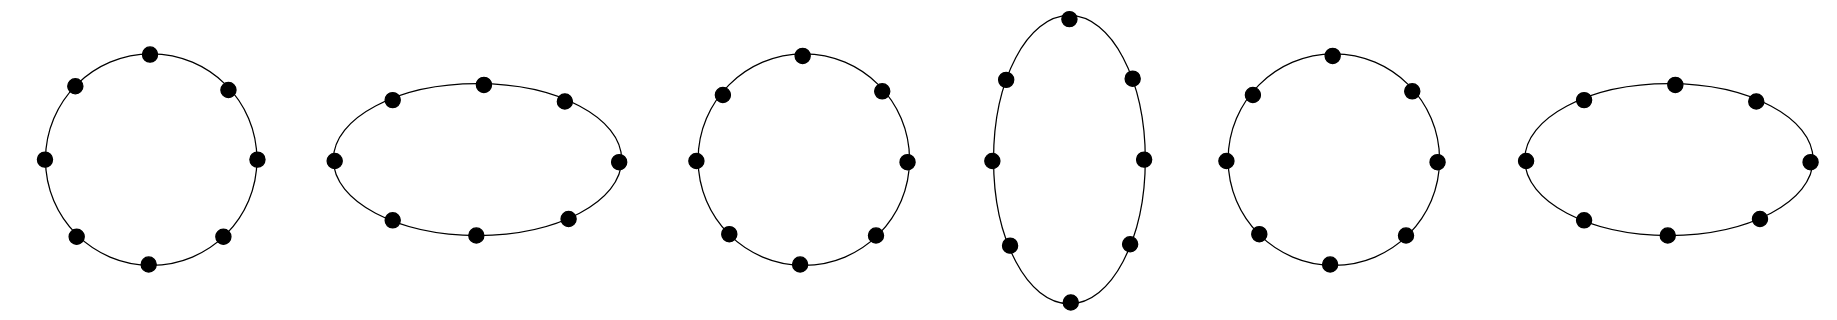
\includegraphics[width = 0.65 \textwidth]{gw-p.png}
\end{figure*}

\subsubsection{$ \times $ polarization}

Setting $ H_\times = 0 $, Eq. \ref{eq:5.21} becomes:
\begin{equation*}
  \frac{d^2 S^1}{dt^2} = - \frac{\omega^2}{2} H_\times e^{i \omega t} S^2
  \qquad \qquad
  \frac{d^2 S^2}{dt^2} = - \frac{\omega^2}{2} H_\times e^{i \omega t} S^1
\end{equation*}
Solving perturbatively in $ H_\times $, at leading order:
\begin{equation}
  S^1(t) = S^1(0) + \frac{1}{2} S^2(0) H_\times e^{i \omega t} + \dots
  \qquad
  S^2(t) = S^2(t) + \frac{1}{2} S^1(0) H_\times e^{i \omega t} + \dots
  \label{eq:5.23}
\end{equation}
This is the same displacement as Eq. \ref{eq:5.22}, but rotated by 45°: to see this, note that $ S^1(t) \pm S^2(t) $ have the same functional expression as Eq. \ref{eq:5.22}. Thus:

\begin{figure*}[h]
  \centering
  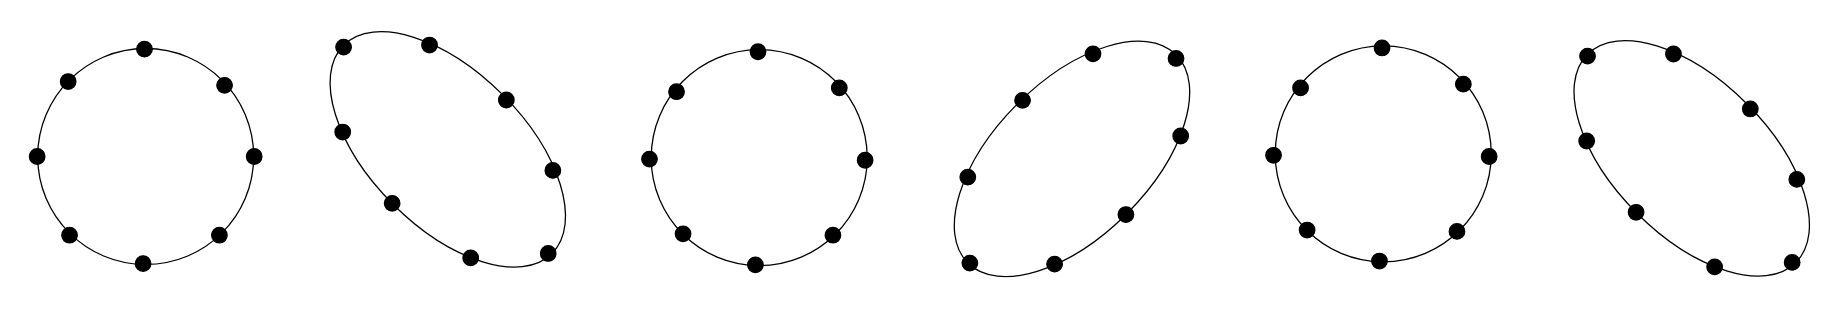
\includegraphics[width = 0.65 \textwidth]{gw-t.png}
\end{figure*}

The general polarization is a linear combination of both: the result is yet an elliptic displacement whose axes rotate, analogously to the circular polarization of light. Interestingly, note that displacements due to gravitational waves are invariant under $ \pi $ rotations, while light polarization, being described by a vector, is invariant under $ 2\pi $ rotations: this reflects the fact that the graviton has spin 2 and the photon has spin 1.

\subsubsection{Gravitational wave detection}

Gravitational wave detectors are interferometers, which bounce light back and forth between two arms. If the gravitational wave propagates perpendicular to the plane of detection, it will shorten one arm and lengthen the other: assuming the arms are aligned with $ x $ and $ y $ axes, the maximum change in length by Eq. \ref{eq:5.22} is $ L' = L (1 \pm H_+ / 2) $, i.e. $ \delta L / L = H_+ / 2 $.
For a typical astrophysical source $ H_+ \sim 10^{-21} $, while for LIGO $ L \sim 3\,\text{km} $, thus $ \delta L \sim 10^{-18} \,\text{m} $: this is smaller than the radius of the proton and extremely difficult to detect, however the first direct measurement of gravitational waves was performed in 2015 and now LIGO and VIRGO detectors have observed a large number of mergers involving black holes and neutron stars.

\begin{figure}[h]
  \centering
  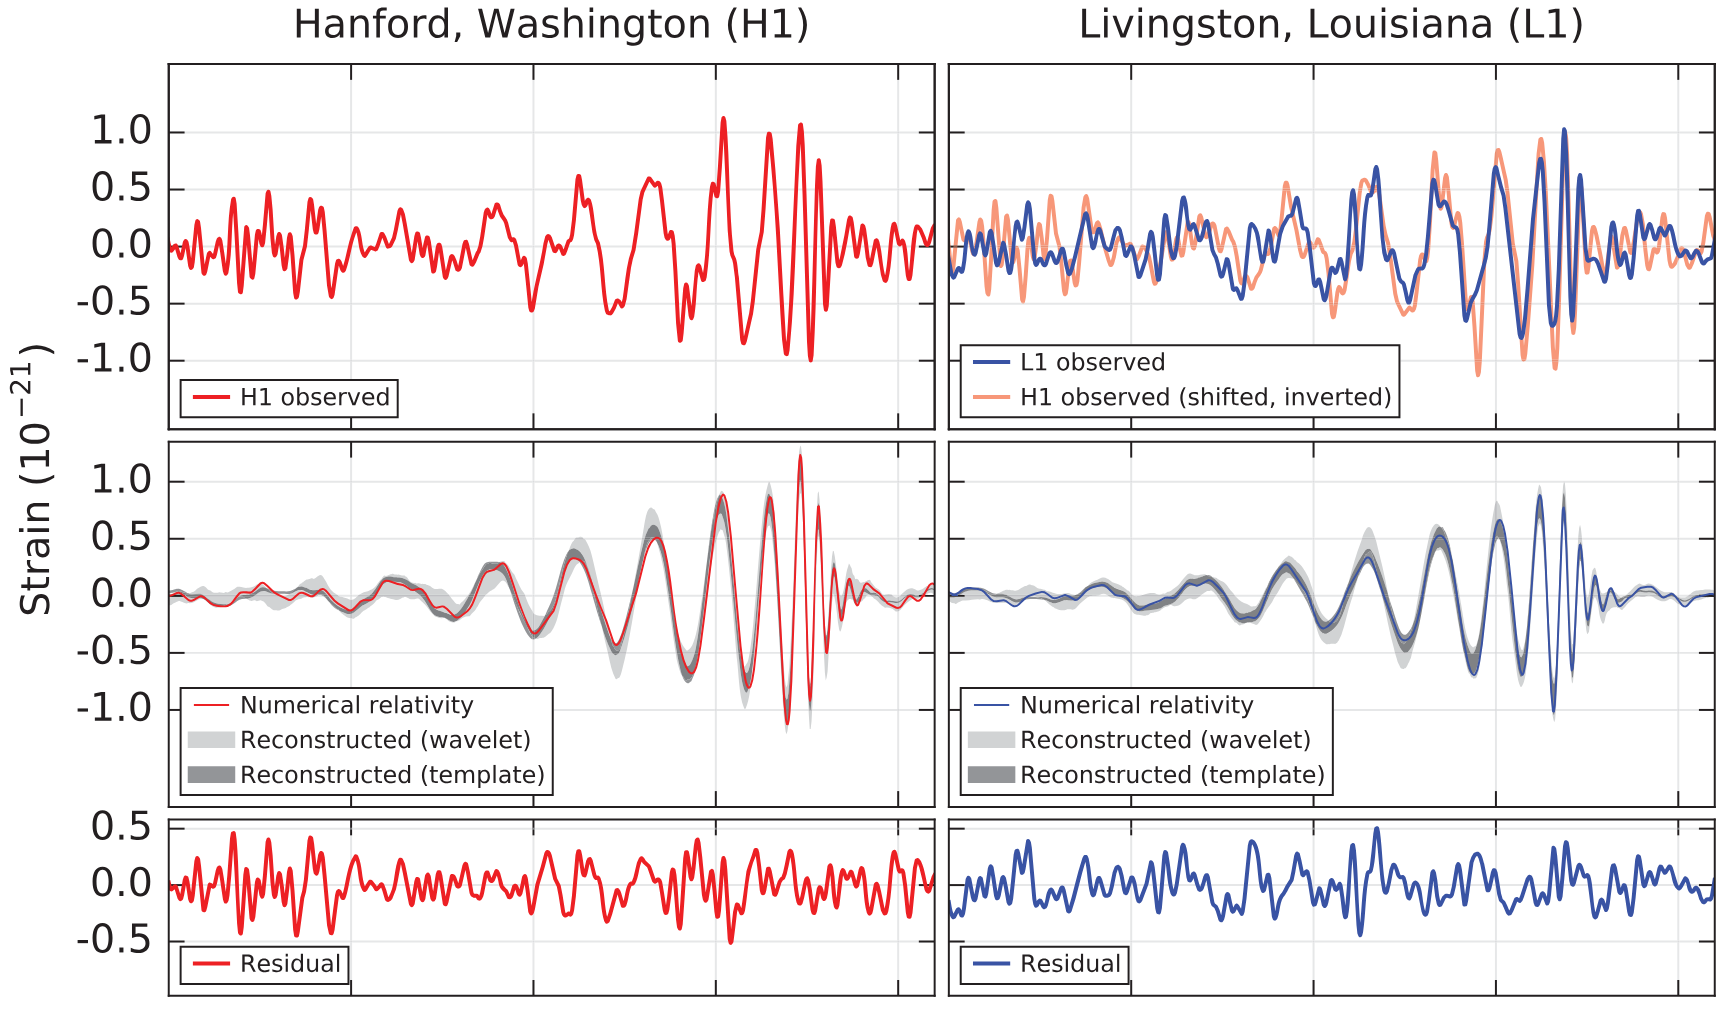
\includegraphics[width = 0.45 \textwidth]{ligo.png}
  \caption{First detection of gravitational waves by LIGO.}
  \label{ligo}
\end{figure}

\subsection{Exact solutions}

Given the found wave-like solution to the linearized field equations, the metric of a wave moving in the positive $ z $ direction takes the form:
\begin{equation}
  ds^2 = -dt^2 + \left( \delta_{ab} + h_{ab}(z - t) \right) dx^a dx^b + dz^2
  \label{eq:5.24}
\end{equation}
with $ a,b = 1,2 $. Being the wave equation linear, any function $ h_{ab}(z - t) $ is a solution: Eq. \ref{eq:5.15} is simply the Fourier decomposition of the general solution.\\
The extreme weakness of gravitational waves makes the linearized metric Eq. \ref{eq:5.1} suitable to describe their properties. However, the wave solution has an extension to the general non-linear field equations. Consider a wave propagating in the positive $ z $ direction and introduce lightcone coordinates:
\begin{equation*}
  u = t - z
  \qquad
  v = t + z
\end{equation*}
Then, consider the plane wave ansatz, also called \textit{Brinkmann metric}:
\begin{equation*}
  ds^2 = -du\,dv + dx^a dx^a + H_{ab}(u) x^a x^b du^2
\end{equation*}
Note that to obtain the linearized metric Eq. \ref{eq:5.24} from Brinkmann metric, one needs some change of coordinates. It is possible to show that Brinkmann metric is Ricci flat for any traceless matrix $ H_{ab}(u) $, hence solving the vacuum Einstein equations:
\begin{equation*}
  R_{\mu \nu} = 0 \quad \Leftrightarrow \quad \tensor{H}{^a_a}(u) = 0 \quad \Leftrightarrow \quad H_{ab}(u) =
  \begin{bmatrix}
    H_{11}(u) & H_{12}(u) \\
    H_{12}(u) & -H_{11}(u)
  \end{bmatrix}
\end{equation*}
The general metric has again two independent polarization states.

\section{Perturbing spacetime}

The gravitational plane wave solution Eq. \ref{eq:5.15} is not realistic, as it is comes from infinity and goes to infinity: in reality, gravitational waves are produced at some point and radiate out. The analogy with Electromagnetism persists: as electromagnetic waves are produced by oscillating charges, gravitational waves are produced by oscillating masses.

\subsection{Green's function}

Recall the linearized Einstein field equations Eq. \ref{eq:5.12}:
\begin{equation*}
  \Box \bar{h}_{\mu \nu} = -16\pi G T_{\mu \nu}
\end{equation*}
which assumes that both $ h_{\mu \nu} $ and $ T_{\mu \nu} $ are small. These are a set of decoupled wave equations.\\
Consider a matter field localized in a spatial region $ \Sigma $, in which a time-dependent energy-momentum source $ T_{\mu \nu}(\ve{x},t) $ is present (ex.: two orbiting black holes): the localization condition then is simply $ T_{\mu \nu}(\ve{x},t) = 0 \,\forall \ve{x} \notin \Sigma $. The question is what the metric $ h_{\mu \nu} $ looks like far away from $ \Sigma $. The solution to Eq. \ref{eq:5.12} outside of $ \Sigma $ can be expressed using the retarded Green's function:
\begin{equation}
  \bar{h}_{\mu \nu}(\ve{x},t) = 4G \int_\Sigma d^3 x'\, \frac{T_{\mu \nu}(\ve{x}',t_r)}{\abs{\ve{x} - \ve{x}'}}
  \qquad t_r \equiv t - \abs{\ve{x} - \ve{x}'}
  \label{eq:5.25}
\end{equation}
Retarded time expresses the causality of the wave equation. This solution satisfies de Donder condition $ \pa^\mu \bar{h}_{\mu \nu} = 0 $ only if $ \pa^\mu T_{\mu \nu} = 0 $, i.e. the energy-momentum tensor is conserved; however, it does not automatically satisfy conditions Eq. \ref{eq:5.19}.\\
Denoting the size of $ \Sigma $ as $ d $ and $ r \equiv \abs{x} $, then approximating:
\begin{equation*}
  \abs{\ve{x} - \ve{x}'} \gg d \,\forall \ve{x}' \in \Sigma
  \quad \Rightarrow \quad
  \abs{\ve{x} - \ve{x}'} = r - \frac{\ve{x} \cdot \ve{x}'}{r} + \dots
  \quad \Rightarrow \quad
  \frac{1}{\abs{\ve{x} - \ve{x}'}} = \frac{1}{r} + \frac{\ve{x} \cdot \ve{x}'}{r^3} + \dots
\end{equation*}
To approximate the energy-momentum tensor, assume that the motion of matter is non-relativistic, so that $ T_{\mu \nu} $ does not change much over the time $ \tau \sim d $ needed to light to cross $ \Sigma $. For example, in the case of two objects orbiting each other with characteristic frequency $ \omega $, then $ T_{\mu \nu} \sim e^{-i \omega t} $ and the non-relativistic condition reads $ d \ll 1/\omega $. Taylor expanding $ T_{\mu \nu} $:
\begin{equation*}
  T_{\mu \nu}(\ve{x}',t_r) = T_{\mu \nu} (\ve{x}', t - r + \ve{x} \cdot \ve{x}' / r + \dots) = T_{\mu \nu}(\ve{x}', t - r) + \dot{T}_{\mu \nu} (\ve{x}', t - r) \frac{\ve{x} \cdot \ve{x}'}{r} + \dots
\end{equation*}
At leading order in $ d/r $, then, the solution becomes:
\begin{equation*}
  \bar{h}_{\mu \nu} (\ve{x},t) \approx \frac{4G}{r} \int_\Sigma d^3 x'\, T_{\mu \nu}(\ve{x}', t - r)
\end{equation*}
The temporal component is:
\begin{equation*}
  \bar{h}_{\mu \nu}(\ve{x}) \approx \frac{4G}{r} E
  \qquad \qquad
  E \equiv \int_\Sigma d^3 x'\, T_{00}(\ve{x}', t - r)
\end{equation*}
This is simply the Newtonian limit; note that there's no time-dependency, as $ \pa^\mu T_{\mu \nu} = 0 $ ensures that the energy $ E $ inside $ \Sigma $ is conserved. Similarly:
\begin{equation*}
  \bar{h}_{0 i}(\ve{x}) \approx - \frac{4G}{r} P_i
  \qquad \qquad
  P_i \equiv - \int_\Sigma d^3 x'\, T_{0 i}(\ve{x}', t - r)
\end{equation*}
Again, the total momentum of matter inside $ \Sigma $ is conserved, hence the absence of time-dependence. Note that it's always possible to choose a rest-frame where matter is stationary, i.e. $ P_i = 0 $ and $ h_{0 i} = 0 $. The motion of matter inside $ \Sigma $ is instead described by $ \bar{h}_{ij} $.

\begin{proposition}
  Far away from the source, the spatial metric takes the form:
  \begin{equation}
    \bar{h}_{ij}(\ve{x},t) \approx \frac{2G}{r} \ddot{I}_{ij}(t - r)
    \qquad \qquad
    I_{ij}(t) \defeq \int_\Sigma d^3 x\, T^{00}(\ve{x},t) x_i x_j
    \label{eq:5.26}
  \end{equation}
  where $ I_{ij}(t) $ is the \textit{quadrupole moment for the energy}.
\end{proposition}
\begin{proof}
  The thesis is equivalent to:
  \begin{equation*}
    \int_\Sigma d^3 x'\, T_{ij}(\ve{x},t) = \frac{1}{2} \ddot{I}_{ij}(t)
  \end{equation*}
  Recalling current conservation $ \pa_\mu T^{\mu \nu} = 0 $:
  \begin{equation*}
    T^{ij} = \pa_k (T^{ik} x^j) - (\pa_k T^{ik}) x^j = \pa_k (T^{ik} x^j) + \pa_0 T^{0i} x^j
  \end{equation*}
  \begin{equation*}
    T^{0i} = \pa_k (T^{0k} x^i) - (\pa_k T^{0k}) x^i = \pa_k (T^{0k} x^i) + \pa_0 T^{00} x^i
    \quad \Rightarrow \quad
    T^{0(i} x^{j)} = \frac{1}{2} \pa_k (T^{0k} x^i x^j) + \frac{1}{2} \pa_0 T^{00} x^i x^j
  \end{equation*}
  Integrating the first over $ \Sigma $, recalling that $ T^{ij} = T^{(ij)} $, and dropping the total spatial derivatives yields the result.
\end{proof}

The physical meaning of Eq. \ref{eq:5.26} is that if a matter distribution is shaken then, after the time needed for signal to propagate, is will affect the metric. Given the linearity of these equations, if matter oscillates at a frequency $ \omega $, then spacetime will create waves at parametrically same frequency.\\
The gauge condition $ \pa^\mu \bar{h}_{\mu \nu} = 0 $ means that $ \pa_0 \bar{h}_{0i} = \pa_j \bar{h}_{ji} $ and $ \pa_0 \bar{h}_{00} = \pa_i \bar{h}_{i0} $. The first equation gives:
\begin{equation*}
  \pa_0 \bar{h}_{0i} = - \frac{2G \hat{x}_j}{r^2} \ddot{I}_{ij}(t - r) - \frac{2G \hat{x}_j}{r} \dddot{I}_{ij}(t - r)
\end{equation*}
where $ \pa_j r = x_j / r \equiv \hat{x}_j $. Note that, though the first term is $ \sim 1/r^2 $ and the second $ \sim 1/r $, the latter has an additional time derivative, i.e. an extra factor of the characteristic source frequency $ \omega $: therefore, the second term dominates for $ r \gg 1/\omega $, i.e. $ r \gg \lambda $ (emitted gravitational waves' wavelength). This is the so-called \textit{far-field zone} or \textit{radiation zone}, and in this regime:
\begin{equation}
  \bar{h}_{0i} \approx - \frac{4G}{r} P_i - \frac{2G \hat{x}_j}{r} \ddot{I}_{ij} (t - r)
  \label{eq:5.27}
\end{equation}
Note that this expression, found integrating the preceding equation, contains an integration constant given by the aforementioned $ P_i $, but it can be set to zero choosing coordinates in which the center of mass of the system is stationary. By analogous reasoning:
\begin{equation}
  \bar{h}_{00} \approx \frac{4G}{r} E + \frac{2G \hat{x}_i \hat{x}_j}{r} \ddot{I}_{ij} (t - r)
  \label{eq:5.28}
\end{equation}

\begin{example}
  Consider two objects of mass $ R $ and separated by a distance $ R $, orbiting in the $ (x,y) $ plane: by Newtonian gravity, the orbit frequency is $ \omega^2 = 2GM / R^3 $. Treating these objects as point particles, their energy density is:
  \begin{equation*}
    T^{00}(\ve{x},t) = M \delta(z) \left[ \delta \left( x - \frac{R}{2} \cos \omega t \right) \delta \left( y - \frac{R}{2} \sin \omega t \right) + \delta \left( x + \frac{R}{2} \cos \omega t \right) \delta \left( y + \frac{R}{2} \sin \omega t \right) \right]
  \end{equation*}
  The quadrupole moment then is:
  \begin{equation*}
    I_{ij} (t) = \frac{MR^2}{2}
    \begin{bmatrix}
      \cos^2 \omega t & \cos \omega t \sin \omega t & 0 \\
      \cos \omega t \sin \omega t & \sin^2 \omega t & 0 \\
      0 & 0 & 0
    \end{bmatrix}
    = \frac{MR^2}{4}
    \begin{bmatrix}
      1 + \cos 2 \omega t & \sin 2 \omega t & 0 \\
      \sin 2 \omega t & 1 - \cos 2 \omega t & 0 \\
      0 & 0 & 0
    \end{bmatrix}
  \end{equation*}
  The resulting metric perturbation is:
  \begin{equation*}
    \bar{h}_{ij}(\ve{x},t) \approx - \frac{2GMR^2 \omega^2}{r}
    \begin{bmatrix}
      \cos 2 \omega t_r & \sin 2 \omega t_r & 0 \\
      \sin 2 \omega t_r & - \cos 2 \omega t_r & 0 \\
      0 & 0 & 0
    \end{bmatrix}
  \end{equation*}
  with $ t_r = t - r $. This gravitational wave propagates approximately radially. To estimate its expected strength:
  \begin{equation*}
    \abs{h_{ij}} \sim \frac{2GMR^2 \omega^2}{r} \sim \frac{G^2 M^2}{Rr}
  \end{equation*}
  Thus, the signal is largest for large masses orbiting very tightly. The most dense objects are black holes, for which $ R_s = 2GM $, so considering two black holes orbiting at $ R \approx R_s $ then $ \abs{h_{ij}} \sim GM / r \sim R_s / r $: black holes of a few solar masses have $ R_s \sim 10\,\text{km} $, so if they are situated in a galaxy a billion light-years away from Earth $ r \sim 10^{21}\,\text{km} $, hence $ \abs{h} \sim 10^{-20} $.
\end{example}

\subsubsection{Multipole expansion}

Comparing to Electromagnetism, recall the first multipoles of the charge distribution $ \rho(\ve{x}) $:
\begin{equation*}
  Q = \int_\Sigma d^3 x\, \rho(\ve{x})
  \qquad
  \ve{p} = \int_\Sigma d^3 x\, \rho(\ve{x}) \ve{x}
  \qquad
  \mathcal{Q}_{ij} = \int_\Sigma d^3 x\, \rho(\ve{x}) \left( 3 x_i x_j - \delta_{ij} x^2 \right)
\end{equation*}
Charge conservation $ \dot{Q} = 0 $ nullifies the monopole contribution to electromagnetic waves. The leading order contribution is that of the dipole:
\begin{equation*}
  \ve{A}(\ve{x},t) \approx \frac{\mu_0}{4\pi} \dot{\ve{p}}(t - r)
\end{equation*}
For gravity, the first multipoles of the energy distribution $ T_{00}(\ve{x}) $ are:
\begin{equation*}
  E = \int_\Sigma d^3 x\, T_{00}(\ve{x})
  \qquad
  \ve{X} = \frac{1}{E} \int_\Sigma d^3 x\, T_{00}(\ve{x}) \ve{x}
  \qquad
  I_{ij} = \int_\Sigma d^3 x\, T_{00}(\ve{x},t) x_i x_j
\end{equation*}
i.e. the total energy, the center of mass (energy) of the distribution and the quadrupole. Energy conservation $ \dot{E} = 0 $ is responsible for the lack of monopole contribution to gravitational radiation. But in contrast to Electromagnetism, the dipole contribution also vanishes due to momentum conservation $ \dot{\ve{P}} = \ve{0} $:
\begin{equation*}
  E \dot{X}_i = \int_\Sigma d^3 x\, (\pa_0 T_{00}) x_i = \int_\Sigma d^3 x\, (\pa_j T_{j0}) x_i = - \int_\Sigma d^3 x\, T_{i0} = P_i
  \quad \Rightarrow \quad
  E \ddot{\ve{X}} = \dot{\ve{P}} = \ve{0}
\end{equation*}
In Electromagnetism, another dipole contribution to the gauge potential is possible:
\begin{equation*}
  \ve{A}(\ve{x},t) = -\frac{\mu_0}{4\pi r} \hat{\ve{x}} \times \dot{\ve{m}}(t - r)
  \qquad \qquad
  \ve{m} \defeq \frac{1}{2} \int_\Sigma d^3 x\, \ve{x} \times \ve{J}(\ve{x})
\end{equation*}
For gravity, there's an equivalent contribution with the analogue of magnetic dipole being:
\begin{equation*}
  J_i = \int_\Sigma d^3 x\, \epsilon_{ijk} x_j T_{0k}
\end{equation*}
This is nothing other than the total angular momentum of the system, thus the dipole contribution to gravitational radiation is nullified by angular momentum conservation $ \dot{\ve{J}} = \ve{0} $ too. The leading order effect for gravitational waves is then the quadrupole.

\subsection{Radiated power}

In the context of Electromagnetism, the power radiated as electromagnetic waves are emitted is easily found defining the Poynting vector $ \ve{S} \defeq \frac{1}{\mu_0} \ve{E} \times \ve{B} $ and, using the dipole approximation, finding \textit{Larmor formula}:
\begin{equation*}
  \mathcal{P} = \int_{\mathbb{S}^2} d^2\ve{r} \cdot \ve{S} = \frac{\mu_0}{6\pi c} \abs{\ddot{p}}^2
\end{equation*}
Analogously, a source emitting gravitational waves loses energy which is carried by them. The problem of finding an equivalent to Larmor formula is that there's no local energy-momentum tensor for gravitational fields, so there's no analogue to the Poynting vector. A possible way forward is to define an energy-momentum tensor $ t_{\mu \nu} $ for gravitatonal waves which, in the linearized theory, obeys $ \pa^\mu t_{\mu \nu} = 0 $: Eq. \ref{eq:4.49} does not allow to do so in a diffeomorphism-invariant way, i.e. in the full non-linear theory $ t_{\mu \nu} $ is not a tensor and in the linearized theory it is not invariant under gauge transformations Eq. \ref{eq:5.9}. It turns out that there are a number of different ways to define such a tensor.

\subsubsection{Fierz-Pauli action}

Recall the Fierz-Pauli action Eq. \ref{eq:5.8} for linearized gravity: viewed as an action describing a spin 2 field propagating through Minkowski spacetime, it can be treated as any classical field theory and used to compute an energy-momentum tensor. In the transverse traceless gauge, i.e. with $ h = 0 $ and $ \pa^\mu h_{\mu \nu} = 0 $, after integration by parts the action becomes:
\begin{equation*}
  \mathcal{S}_{\text{FP}} = - \frac{1}{8\pi G} \int d^4 x\, \frac{1}{4} \pa_\rho h_{\mu \nu} \pa^\rho h^{\mu \nu}
\end{equation*}
This looks like the action for a set of massless scalar fields, hence the energy dentity takes the schematic form:
\begin{equation*}
  t^{00} \sim \frac{1}{G} \dot{h}_{\mu \nu} \dot{h}^{\mu \nu}
\end{equation*}
There are gradient terms too, but, due to the wave equation, they contribute as time derivatives. Note that $ t^{0i} $ scales in the same way. In the transverse traceless gauge, Eq. \ref{eq:5.26} becomes:
\begin{equation*}
  h_{ij}(\ve{x},t) \sim \frac{G}{r} \ddot{\mathcal{Q}}(t - r)
  \qquad \qquad
  \mathcal{Q}_{ij} \equiv I_{ij} - \frac{1}{3} I_{kk} \delta_{ij}
\end{equation*}
where $ \mathcal{Q}_{ij} $ is the traceless part of the quadrupole moment $ I_{ij} $. The energy density carried by gravitational waves should then be:
\begin{equation*}
  t^{00} \sim \frac{G}{r^2} \dddot{\mathcal{Q}}_{ij}^2
\end{equation*}
Integrating over a sphere at large distance suggests that $ \mathcal{P} \sim G \dddot{\mathcal{Q}}_{ij}^2 $, and this is indeed correct, as it can be shown that:
\begin{equation}
  \mathcal{P}(t) = \frac{G}{5} \dddot{\mathcal{Q}}_{ij}(t_r) \dddot{\mathcal{Q}}^{ij}(t_r)
  \label{eq:5.29}
\end{equation}
This is the \textit{quadrupole formula} and it is analogous to Larmor formula. Note that $ r $ is the distance at which the gravitational waves are observed.

\subsubsection{Conceptual issues}

Although Eq. \ref{eq:5.29} is indeed correct, as the 1993 Nobel prize was awarded for data in agreement with it, there remains some conceptual issues in the definition of $ t_{\mu \nu} $, which can be improved.\\
First, note that the definition of $ t_{\mu \nu} $ from the Fierz-Pauli action suffers a number of ambiguities: if one attempts to compute it as the Noether currents associated to spacetime translations, the result is neither symmetric nor gauge invariant, but this is also true for Maxwell theory. An idea could be to add a term: $ t_{\mu \nu} \mapsto t_{\mu \nu} + \pa^\rho \Theta_{\rho \mu \nu} $, with $ \Theta_{\rho \mu \nu} = - \Theta_{\mu \rho \nu} $ as to not violate current conservation; such a term would make $ t_{\mu \nu} $ symmetric, but still not gauge invariant.\\
A different approach is to interpret the lack of energy conservation for matter fields as energy transferred to the gravitational field. Although covariant conservation is not actual conservation for $ T_{\mu \nu} $, it can be rewritten as:
\begin{equation*}
  0 = \na_\mu \tensor{T}{^\mu_\nu} = \frac{1}{\sqgm} \pa_\mu (\sqgm\, \tensor{T}{^\mu_\nu}) - \Gamma^\rho_{\mu \nu} \tensor{T}{^\mu_\rho} = \frac{1}{\sqgm} \pa_\mu (\sqgm\, \tensor{T}{^\mu_\nu}) - \frac{1}{2} \pa_\nu g_{\mu \rho} T^{\mu \rho}
\end{equation*}
where the symmetry of $ T_{\mu \nu} $ was used. Note that $ \Gamma^\rho_{\mu \nu} $ reduces to $ g_{\mu \rho , \nu} $ only when $ \nu $ is down: this reflects that this equation is non-covariant. Using the field equations:
\begin{equation*}
  \pa_\mu (\sqgm\, \tensor{T}{^\mu_\nu}) = \frac{1}{16\pi G} \sqgm\, \pa_\nu g_{\mu \rho} \left( R^{\mu \rho} - \frac{1}{2} R g^{\mu \rho} \right) = \frac{1}{16\pi G} \sqgm\, \pa_\nu g_{\mu \rho} R^{\mu \rho}
\end{equation*}
The idea is to express this equation as $ \pa_\mu (\sqgm\, \tensor{T}{^\mu_\nu}) = - \pa_\mu (\sqgm\, \tensor{t}{^\mu_\rho}) $, for some $ \tensor{t}{^\mu_\nu} $ referred to as \textit{Landau-Lifshitz pseudotensor}: this suggests that the sum of matter energy $ \tensor{T}{^\mu_\nu} $ and gravitational energy $ \tensor{t}{^\mu_\nu} $ is conserved, however it would be coordinate-dependent as $ \tensor{t}{^\mu_\nu} $ is not a real tensor.\\
The final approach assumes that $ t_{\mu \nu} $ is quadratic in $ h_{\mu \nu} $, so, keeping $ g_{\mu \nu} = \eta_{\mu \nu} + h_{\mu \nu} $, expand the Einstein field equations to second order:
\begin{equation*}
  \left[ R_{\mu \nu} - \frac{1}{2} R g_{\mu \nu} \right]^{(1)} + \left[ R_{\mu \nu} - \frac{1}{2} R g_{\mu \nu} \right]^{(2)} = 8\pi G T_{\mu \nu}
  \quad \Leftrightarrow \quad
  \left[ R_{\mu \nu} - \frac{1}{2} R g_{\mu \nu} \right]^{(1)} = 8\pi G (T_{\mu \nu} + t_{\mu \nu})
\end{equation*}
where superscripts $ (n) $ denote a restriction to terms of order $ h^n $. The gravitational energy-momentum non-tensor thus is:
\begin{equation*}
  t_{\mu \nu} = - \frac{1}{8\pi G} \left[ R_{\mu \nu} - \frac{1}{2} R g_{\mu \nu} \right]^{(2)} = - \frac{1}{8\pi G} \left[ R^{(2)}_{\mu \nu} - \frac{1}{2} R^{(2)} \eta_{\mu \nu} - \frac{1}{2} R^{(1)} h_{\mu \nu} \right]
\end{equation*}
Far away from the source $ R^{(1)} $ can be neglected, since it vanishes by the equations of motion (at linear order), so:
\begin{equation}
  t_{\mu \nu} = - \frac{1}{8\pi G} \left[ R^{(2)}_{\mu \nu} - \frac{1}{2} R^{(2)} \eta_{\mu \nu} \right]
  \label{eq:5.30}
\end{equation}
The linearized Bianchi identity is $ \pa^\mu \left[ R_{\mu \nu} - \frac{1}{2} R g_{\mu \nu} \right]^{(1)} = 0 $, hence, far away from sources, i.e. $ T_{\mu \nu} = 0 $, necessarily $ \pa^\mu t_{\mu \nu} = 0 $ as befits a conserved current. However, $ t_{\mu \nu} $ is still not gauge invariant.

\subsubsection{Gauge invariance}

Although none of the defined $ t_{\mu \nu} $ is gauge invariant, it is still possible to extract a gauge-invariant quantity from it, which has physical meaning.\\
First, if the spacetime is asymptotically Minkowski, it could be possible to integrate $ t^{00} $ on an infinite spatial hypersurface, obtaining the so-called \textit{ADM energy}, which is shown to be constant in time and gauge.invariant. Alternatively, one could integrate $ t^{0i} $ on a sphere at $ \mathcal{I}^+ $, yielding the so-called \textit{Bondi energy}, which is gauge-invariant and time-dependent, and it can be defined in the full non-lnear theory too.\\
Moreover, consider that, like any other waves, gravitational waves vary over some typical length $ \lambda $. Thus, averaging over these oscillations is possible by:
\begin{equation*}
  \braket{t_{\mu \nu}} \defeq \int_V d^4 y\, W(x - y) t_{\mu \nu}(y)
\end{equation*}
where $ V $ is a spacetime region of typical size $ a $ and $ W \in \mathcal{C}^{\infty}(V) : \int_V d^4 x\, W(x) = 1 \,\land\, W\vert_{\pa V} = 0 $. This integral averages total derivatives as $ \braket{\pa X} \sim 1/a $, so $ \braket{X \pa Y} = - \braket{Y \pa X} + o(1/a) $. Then:
\begin{equation}
  \braket{t_{\mu \nu}} = \frac{1}{32\pi G} \braket{\pa_\mu h_{\rho \sigma} \pa_\nu h^{\rho \sigma}}
  \label{eq:5.31}
\end{equation}
This is indeed a conserved quantity:
\begin{equation*}
  \pa^\mu \braket{t_{\mu \nu}} = \frac{1}{32\pi G} \braket{(\Box h_{\rho \sigma}) \pa_\nu h^{\rho \sigma} + \frac{1}{2} \pa_\nu (\pa_\mu h_{\rho \sigma} \pa^\mu h^{\gamma \sigma})} = 0
\end{equation*}
as the first term vanishes by equations of motion and the second yields a negligible total derivative. Under a gauge transformation like Eq. \ref{eq:5.9}:
\begin{equation*}
  \delta \braket{t_{\mu \nu}} = \frac{1}{16\pi G} \braket{\pa_\mu h_{\rho \sigma} \pa_\nu (\pa^\rho \xi^\sigma + \pa^\sigma \xi^\rho)} = \frac{1}{16\pi G} \braket{\pa_\mu \pa^\rho h_{\rho \sigma} \pa_\nu \xi^\sigma + \pa_\mu \pa^\sigma h_{\rho \sigma} \pa_\nu \xi^\rho} + o(a^{-1}) = o(a^{-1})
\end{equation*}
where, after integration by parts, de Donder gauge condition $ \pa^\rho h_{\rho \sigma} = 0 $ was invoked. Hence, $ t_{\mu \nu} $ is almost gauge-invariant, and it is properly gauge-invariant if $ a \rightarrow \infty $, i.e. if the averaging is over all of spacetime. The power emitted by a gravitational wave at infinity is:
\begin{equation*}
  \mathcal{P} = \int_{\mathbb{S}^2_{\infty}} d^2 x\, \hat{n}_i \braket{t^{0i}}
\end{equation*}
with $ \hat{n}_i $ a normal versor to $ \mathbb{S}^2_{\infty} $. This indeed gives Eq. \ref{eq:5.29}.

\subsubsection{Orders of magnitude}

\paragraph{Black holes}

Consider two masses $ M $, separated by a distance $ R $ and orbiting each other with frequency $ \omega $. Newtonian gravity approximation gives:
\begin{equation*}
  \omega^2 R \sim \frac{GM}{R^2}
\end{equation*}
The quadrupole is $ \mathcal{Q} \sim M R^2 $, hence $ \dddot{\mathcal{Q}} \sim \omega^3 M R^2 $, and the emitted power scales as:
\begin{equation*}
  \mathcal{P} \sim G \dddot{\mathcal{Q}}^2 \sim \frac{G^4 M^5}{R^5}
\end{equation*}
Returning to SI units, $ [G] = M^{-1} L^3 T^{-2} $ and, for a black hole, $ R_s = 2GM / c^2 $, thus:
\begin{equation*}
  \mathcal{P} = \left( \frac{R_s}{R} \right)^5 L_{\text{p}}
\end{equation*}
where the \textit{Plank luminosity} is defined as:
\begin{equation*}
  L_{\text{p}} \equiv \frac{c^5}{G} \approx 3.6 \cdot 10^{52} \,\text{J}\,\text{s}^{-1}
\end{equation*}
To get a sense of scale, the Sun emits $ L_{\odot} \approx 10^{-26} L_{\text{p}} $ and the Milky Way, with $ 10^{11} $ stars, emits $ L \approx 10^{-15} L_{\text{p}} $. Moreover, in the visible Universe there are roughly $ 10^{10} $ galaxies, so all the stars of the visible Universe shine with $ L \approx 10^{-5} L_{\text{p}} $. Yet, when two black holes spiral towards each other, when their separation is comparable to their Schwarzschild radius, they emit in gravitational waves $ 10^5 $ times the energy emitted by all the stars of the visible Universe.

\paragraph{Solar System}

If two objects with masses $ M_1 \gg M_2 $ orbit each other, then their gravitationally-radiated power is:
\begin{equation*}
  \mathcal{P} \sim \frac{G^4 M_1^3 M_2^2}{R^5}
\end{equation*}
Considering Jupiter, which has $ M \sim 10^{-3} M_{\odot} $ and orbits at $ R \approx 10^9\,\text{km} $ from the Sun, which has $ R_s \approx 3\,\text{km} $:
\begin{equation*}
  \mathcal{P} \approx 10^{-50} L_{\text{p}} \approx 10^{-24} L_{\odot}
\end{equation*}
This is completely negligible.

\paragraph{Human body}

Consider a human being shaking its arms around. The mass of a human arm is a few kg and moves a distance of around $ 1\,\text{m} $ with a frequency $ \omega \sim 1\,\text{Hz} $, so $ \mathcal{Q} \approx 1\,\text{kg}\,\text{m}^2 $ and $ \dddot{\mathcal{Q}} \approx 1\,\text{kg}\,\text{m}^2\,\text{s}^{-3} $, hence the gravitationally-radiated power is:
\begin{equation*}
  \mathcal{P} \sim \frac{G \dddot{\mathcal{Q}}^2}{c^5} \approx 10^{-52}\,\text{J}\,\text{s}^{-1 \approx 10^{-52}\,\text{J}\,\text{s}^{-1}}
\end{equation*}
Suppose the existence of gravitons with $ E = \hbar\omega $: to produce a single graviton with $ \omega = 1\,\text{Hz} $, i.e. $ E \approx 10^{-34}\,\text{J} $, a human needs to shake its arms around for $ t \approx 10^{18}\,\text{s} $: this is approximately the age of the Universe.










